% !TeX spellcheck = en_GB
\section{Question 1}

\subsection{A)}
\begin{quote}
	\textit{"Consider	Apache	Flink: \url{https://flink.apache.org}.	You	should	characterize	this	system,	describe	how	it	can	be	used	in	the	context	of	the	Lambda	architecture	and	compare	it	with	systems	you	have	used	during	your	projects."}
\end{quote}

\newpar Apache Flink(from here just Flink) is a streaming dataflow engine. It works in a distributed setting and makes analysis of streaming data (data in motion), and batch data(data at rest) analysis easier. It incorporates multiple other systems, for machine learning, graph-analysis, and more. To further characterize Flink I will use the characterization model presented in the course.

\newpar \textbf{Datamodel:} Flink works on event-based streams of data. The specific format it works in is Java and Scala embedded objects. By allowing objects of defined languages it is easy to incorporate Flink with already existing systems, that uses these languages. These streams can either be infinite such as a sensor which continuously sends data, or finite such as a file.

\newpar \textbf{Partition Management:} To be able to scale flink partitions the computations on multiple nodes, which can be placed on the same server or distributed on multiple machine on a network. Opposed to working with data in rest, where the partitioning is based on the data, Flink works with streams and as such, partitions the computations instead and sends the events between such computation nodes. Flink therefore tries to optimize the placement of the operations, such that the overhead of sending the events through the network is minimized\cite{official-flink}.

\newpar \textbf{Failure handling:} Flink supports replaying of a stream to be able to recover from failures, that is if a failure occurs the stream is replayed from the last checkpoint.

The checkpoint mechanism is different from what most other big data systems use as a fallback mechanism. The state of the nodes is periodically persistent on HDFS or in memory, such that in case of a failure replaying from that checkpoint is possible. The system is based on the snapshot algorithm by Chandy and Lamport, such that the checkpoint is consistent across distributed nodes, and it is not necessary to duplicate information. The computation between checkpoints either succeeds or fails as a whole, and is then persistet as the new checkpoint. The approach also handles the problem that is, if a computation fails, on an infinite stream, it is not feasible to recalculate the entire computation again. Once all data has flown through the barrier/checkpoint the computation is done. The flow of the events happen in a DAG like structure which also means that the consistency is strong, since it is not possible to access an event which has not been through all the operations before that access.

This technique also separates the responsibility of flow control and throughput control, since changing the frequency of checkpoints does not alter the results of the stream.

\newpar \textbf{Batch and Stream Processing:} Flink provides two APIs, one for batch analysis and stream analysis. Since Map-Reduce streams HDFS files to do batch processes, Flink has implemented batch processing as a special case of stream-processing, greatly simplifying the process. The only difference is that while streaming data is infinite, batch data is finite. The two API's can be used from Java or Scala, and provide a Java-Streams-Like interface, where it is easy to do typical SQL commands, such as where, grouping, sum and so on. Furthermore Flink has made it possible to easily define a window of the stream to allow for more sophisticated analysis.

Flink provides Pipelining to make nodes able to concurrently work on different tasks, even on different machines.

\newpar \textbf{Throughput:} Flink prides itself with being low latency by offloading some of the batch processing to the stream processing. What the streaming analysis does for low latency the ability to send information quickly forth to batch analysis, as well as the ability to scale vertically allows for high throughput. 

On data-artisan.com\footnote{ \url{http://data-artisans.com/wp-content/uploads/2015/08/grep_throughput.png}} a graph of the throughput of different big data system is made. On figure \ref{fig:flink_bench} the graph can be seen. The strengths of Flink become very apparent, and as we can see in this case the throughput is many times faster than for example storm, which is also known for its high throughput. Flink even has a lower latency, than any of the other measured frameworks.

\begin{figure}[H]
	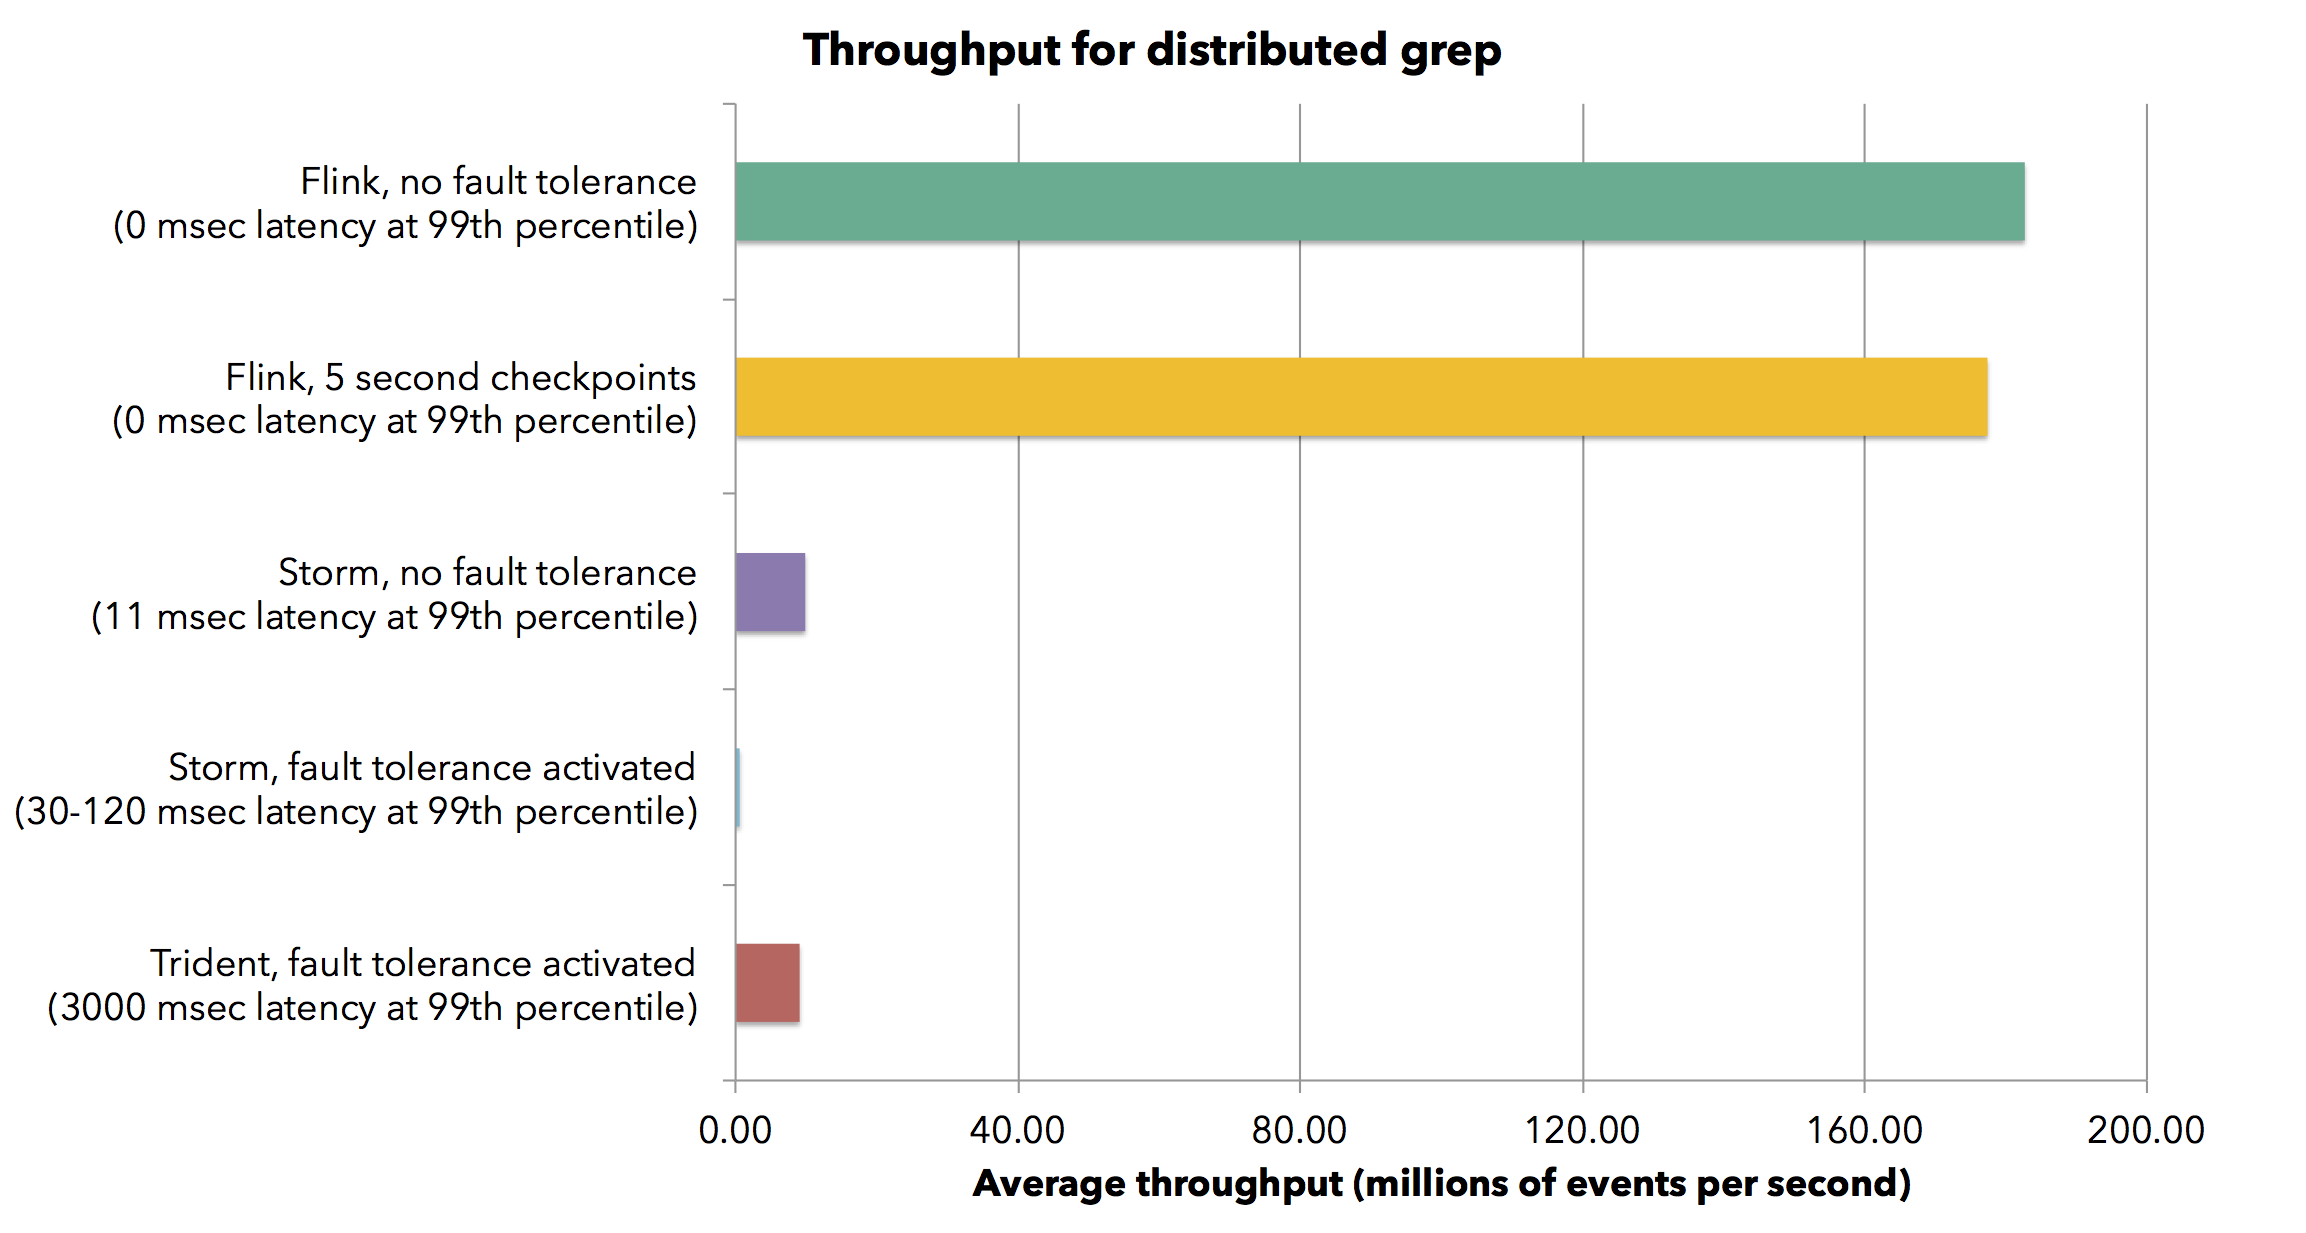
\includegraphics[width=\linewidth]{figures/flink_throughput.png}
	\caption{A graph showing the performance of different big data processing frameworks.}
	\label{fig:flink_bench}
\end{figure}

\newpar Interestingly enough Flink has a lot of comparisons to the Lambda architecture. The Lambda introduced in the course, is separated into the following stages, the data sources, the master dataset, the serving layer, the speed layer and the queries. At the serving layer, batch views are computed, and similarly at the speed layer streaming analysis is done, and therefore it becomes quite clear that Flink naturally fits the lambda architecture by being able to be the main framework for each of these layers. Further more, since Flink allows the same code for streaming analysis to batch analysis this would greatly increase the effectiveness of the developers. Flink also builds on top of HDFS and therefore automatically works with a distributed master dataset.

\newpar For project 2 and 3, we could have made both batch jobs and streaming jobs, but decided to only develop batch jobs. Most of our batch jobs are made out of logic which could be expressed as -\texttt{where}, -\texttt{join} and -\texttt{groupby} statements which are available with Flink. Therefore it would be possible to have written the batch views with the Flink APIs, and have gained higher parallelism, and furthermore had the ability to with ease introduce a speed layer which could do similar calculations. 

\cite{official-flink}
\cite{data-artisan-flink}
\cite{confluent-flink}
\subsection{B)}
\begin{quote}
		\textit{"You	are	asked	to	store	a	master	data	set	of	80	GB	given	to	you	as	an	XML	file.	Why	is	the	XML	data	format	problematic	when	working	with	Map-Reduce?	Would	a	format	transformation	from	XML	to	JSON	be	helpful?	Would	a	transformation	from	XML	to	CSV	be	helpful?	How	would	you	store	this	master	data	set?	Explain	your	answers"}
\end{quote}
The XML format is in a tree structure, and might not be easily partitioned into smaller parts, which can be distributed among the data nodes of the storage system that Map-Reduce works on. Furthermore XML is also a very verbose format and therefore data will take up more space which will make the computations somewhat slower and require more space on the server, even though Hadoop of course handles this quite fine, less space use is always good to be preferred when the available information is the same. 

Transforming the data to JSON would mostly help with the amount of data, since JSON is less verbose than XML. JSON is still a tree-structure language and therefore partitioning would still be difficult especially because JSON objects do not specify a start and an end tag it can actually be more difficult to split up than XML. 

CSV on the other hand is flat data structure and therefore is easily partitioned per line and therefore allow map-reduce to work on multiple processes, greatly increasing performance. Furthermore CSV has the advantage that it is easy to extend the input with more columns.

Another possibility that we have used in Project 2 is to use a binary format. We used the serialization framework Avro\footnote{\url{https://avro.apache.org/}} for this. By choosing to use a binary format, you can represent numbers as numbers therefore cutting down on the needed space. Furthermore if done properly it is still possible to make the format flat. This approach of course requires more work to be done, and also enforces a scheme on the data, which makes it more difficult to extend the system later.

\newpar For project 3 we converted the data to a CSV format and stored it using Hive since it was well integrated. Hive stores the CSV data as distributed files on HDFS but uses an abstraction layer which makes the access seem like a regular database access. Hive allowed us to make all the views we needed and therefore it seemed like a good choice to store the data. 

In project 2 we stored the data directly on HDFS, and used Map-Reduce to make our views, and in this case using Avro serialization of the data worked quite well, since it allowed us to work with data as objects like any other Java program. Therefore it is difficult to conclude which specific approach should be taken and very much depends on the data and what the purpose of the system is.

It is important to notice that as soon as one transforms data, it per definition becomes derived data. Therefore, the master data set will be derived, which puts a question on what happens to the primary data. I will argue that a transformation can be done from XML to CSV, which allows one to go through a similar process which converts the resulting CSV back into XML data which, even though is not the same data, is equal to the primary data, and therefore just keeping the CSV and not the primary data is enough. If it is not possible to derive the original data from the master data set, then the approach to storing the primary data should be up to the goal of the data. If the goal of the system can change then it could be important to have a backup of the data, but if the goal is clear cut then it might not matter.\todo{check om det her overhovedet er ok}

\subsection{C)}
\begin{quote}
	\textit{"Describe	pros	and	cons	of	using	the	Hadoop	ecosystem,	based	on	the	lessons	you	learnt	from	project	2	and	project	3."}
\end{quote}

The Hadoop ecosystem, has changed the industry, and how it looks at data in general. By going from a restricted structured boxed view, the big data movement tries to break these boundaries but it is still in its youth. The relational databases go back to the 1970s and have had many years to polish its rough edges and making it easily available to developers. The big data movement is still trying to do this and most frameworks in the Hadoop data system exactly tries to sell it self as easy to use, but in my experience most of these systems still have a high learning curve. Furthermore setting up a server with a Hadoop ecosystem requires a lot of time. Systems like Horton tries to make this process easier by creating a single entrypoint for organizing and managing a large amount of the different hadoop frameworks. 

\newpar Another con is that integrating different frameworks is often difficult. Since there does not exist a standard often times frameworks are made to integrate well with other specific frameworks, but if it is desired to integrate with another system then the developers are often left to figure out how and if it is possible themselves.

For small systems, or embedded systems where it is known that the amount of data will never surpass a low limit, the overhead of using big data technologies is also often not worth it. Then using relational database systems, can be enough 

A lot of the frameworks have a lot of overhead on what they do, even though they scale better. If you know you will never store a lot of data, or want it to be available on the device of the user, going with a SQLlite or a system specific Relational Database would be smarter.

\newpar That said, the Hadoop ecosystem really shines when it comes to large amounts of data. A lot of businesses saw a huge rise in the amount of data they save through the 2000s and now that processors were nearing their clock speed limit, being able to to scale systems vertically were very important. The Hadoop ecosystem is build around concepts of being able to abstract the distributiveness of the data away and allow developers to write code which automatically would scale to an arbitrary amount of machines. Even in the case of machine breakdowns the frameworks of Hadoop will handle it and be able to replay, reroute, or abandon the process, and the developers are able to specify which approach should be taken as to how to restore the data of that node.

\newpar To conclude on this it becomes obvious that if a system is going to scale, it is a good idea to use the Hadoop ecosystem since other systems might not be able to handle the same amounts of data, but if the system is of limited scale, the overhead of using the hadoop ecosystem is quite high.
